% Hyperion: how it works, and where Rust helps.
%
% Compile with:   pdflatex hyperion-explained.tex   (run it twice for the table of contents)
% Needs only packages that ship with a standard TeX Live / MiKTeX install:
%   geometry, hyperref, listings, xcolor, booktabs, enumitem, tikz, lmodern.

\documentclass[11pt,a4paper]{article}

\usepackage[T1]{fontenc}
\usepackage[utf8]{inputenc}
\usepackage{lmodern}
\usepackage[margin=2.5cm]{geometry}
\usepackage{xcolor}
\usepackage{booktabs}
\usepackage{enumitem}
\usepackage{listings}
\usepackage{tikz}
\usetikzlibrary{arrows.meta,positioning,fit,backgrounds}
\usepackage[colorlinks=true,linkcolor=teal!60!black,urlcolor=teal!60!black]{hyperref}

\setlist{itemsep=2pt, topsep=4pt}
\setlength{\parskip}{0.55em}
\setlength{\parindent}{0pt}

\definecolor{codebg}{gray}{0.96}
\definecolor{kw}{RGB}{140,60,150}
\definecolor{cm}{RGB}{90,120,90}
\definecolor{str}{RGB}{170,90,30}

\lstdefinelanguage{Rust}{
  keywords={as,break,const,continue,crate,else,enum,extern,false,fn,for,if,impl,in,let,loop,match,mod,move,mut,pub,ref,return,self,Self,static,struct,super,trait,true,type,unsafe,use,where,while,async,await,dyn},
  keywordstyle=\color{kw}\bfseries,
  ndkeywords={Option,Some,None,Result,Ok,Err,Vec,String,Arc,Mutex,Duration,Instant},
  ndkeywordstyle=\color{teal!60!black},
  comment=[l]{//},
  commentstyle=\color{cm}\itshape,
  morestring=[b]",
  stringstyle=\color{str},
}
\lstset{
  language=Rust,
  basicstyle=\ttfamily\small,
  backgroundcolor=\color{codebg},
  frame=single,
  rulecolor=\color{gray!40},
  breaklines=true,
  columns=fullflexible,
  keepspaces=true,
  aboveskip=0.8em,
  belowskip=0.4em,
  captionpos=b,
  xleftmargin=0.5em,
  xrightmargin=0.5em,
}

\newcommand{\code}[1]{\texttt{#1}}
\newcommand{\file}[1]{\texttt{#1}}

\newenvironment{callout}[1]{%
  \par\medskip\noindent\hrule\vspace{0.4em}\noindent\small\textbf{#1.}\ \ignorespaces
}{%
  \par\vspace{0.3em}\noindent\hrule\medskip
}

\title{\textbf{Hyperion}\\[0.3em]\large How the project works, and where Rust actually helps}
\author{}
\date{}

\begin{document}
\maketitle
\tableofcontents
\bigskip

% ---------------------------------------------------------------------------
\section{What Hyperion is}

Hyperion is a live system resource monitor: CPU, GPU, memory, storage and network, drawn as
graphs you can rearrange, resize, theme, and tear off into their own windows. It is written
in Rust, with an immediate-mode GUI library called \emph{egui}.

The primary target is Linux on the Hyprland compositor (Wayland). It also has to run on
Debian-family systems (the Mint/Cinnamon X11 machine has been the real test), and Windows and
Android ports are planned for later.

\paragraph{Measured footprint.} On the development machine (Ryzen 5 3600, RX 6600), with the
window visible and default settings (1\,s refresh, 60\,s of history), averaged over 20\,s:

\begin{center}
\begin{tabular}{lr}
\toprule
Metric & Value \\
\midrule
CPU & 0.55\% of one core \\
GPU & 0.27\% \\
Resident memory & about 80\,MB \\
Threads & 16 \\
Release binary & 13\,MB, links only libc, libm and libgcc \\
\bottomrule
\end{tabular}
\end{center}

These are single-machine numbers from one run, not a benchmark suite. Section~\ref{sec:honest}
discusses what they do and do not say about Rust.

% ---------------------------------------------------------------------------
\section{The big picture}

The most important design decision is a split into two threads that never block each other:

\begin{itemize}
  \item A \textbf{sampler thread} reads the kernel's files, does the arithmetic, and writes
        the results into a shared store.
  \item The \textbf{UI thread} only ever \emph{reads} that store and draws it. It never touches
        \file{/proc} or \file{/sys}.
\end{itemize}

\begin{figure}[h]
\centering
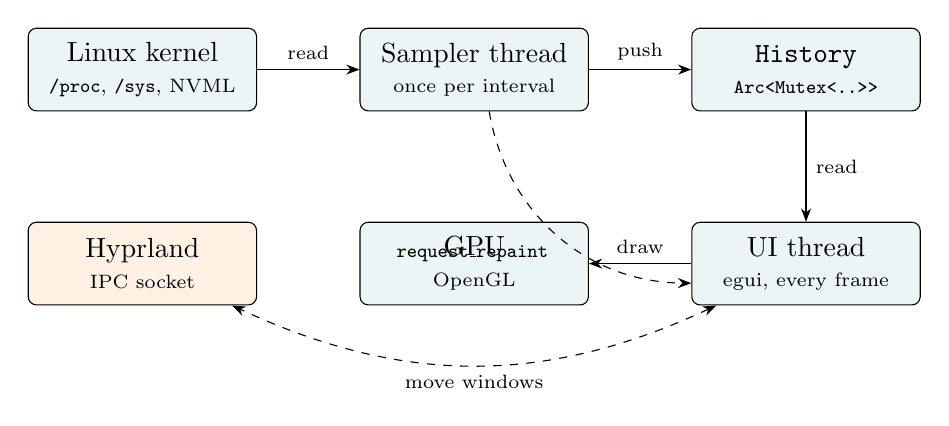
\begin{tikzpicture}[
    >=Stealth,
    box/.style={draw, rounded corners=3pt, align=center, minimum width=2.9cm, minimum height=1.05cm, fill=teal!8},
    side/.style={draw, rounded corners=3pt, align=center, minimum width=2.9cm, minimum height=1.05cm, fill=orange!10},
    node distance=1.0cm and 1.3cm,
    lbl/.style={font=\scriptsize, align=center}
]
  \node[box] (kernel) {Linux kernel\\[-1pt]\scriptsize \code{/proc}, \code{/sys}, NVML};
  \node[box, right=of kernel] (sampler) {Sampler thread\\[-1pt]\scriptsize once per interval};
  \node[box, right=of sampler] (hist) {\code{History}\\[-1pt]\scriptsize \code{Arc<Mutex<..>>}};
  \node[box, below=1.4cm of hist] (ui) {UI thread\\[-1pt]\scriptsize egui, every frame};
  \node[box, left=of ui] (gpu) {GPU\\[-1pt]\scriptsize OpenGL};
  \node[side, left=of gpu] (hypr) {Hyprland\\[-1pt]\scriptsize IPC socket};

  \draw[->] (kernel) -- node[lbl, above] {read} (sampler);
  \draw[->] (sampler) -- node[lbl, above] {push} (hist);
  \draw[->] (hist) -- node[lbl, right] {read} (ui);
  \draw[->] (ui) -- node[lbl, above] {draw} (gpu);
  \draw[<->, dashed] (ui) to[bend left=25] node[lbl, below] {move windows} (hypr);
  \draw[->, dashed] (sampler) to[bend right=40] node[lbl, below left] {\code{request\_repaint}} (ui);
\end{tikzpicture}
\caption{Data flows left to right. The dashed arrows are signals and window control, not data.}
\end{figure}

Why this matters in practice: reading a file can stall (a slow disk, a sensor that takes a
moment to answer). If that happened on the UI thread, the whole window would freeze. Because
the work is on another thread, the worst case is that a graph gets one late point.

\begin{callout}{Web analogy}
Think of the sampler as a background worker (a web worker, or a cron job writing to a cache),
and \code{History} as the cache. The UI is the page that renders from the cache and never
calls the slow backend itself.
\end{callout}

% ---------------------------------------------------------------------------
\section{A tour of the source}

The whole project is about 9,600 lines of Rust, including the tests that live next to the code
they test. Roughly:

\begin{center}
\small
\begin{tabular}{@{}p{3.6cm}p{9.6cm}r@{}}
\toprule
Module & Job & Lines \\
\midrule
\file{sampler/} & Reads CPU, memory, disk, network, GPU and sensors. One file per source; \file{gpu/} has a backend each for AMD, Intel and NVIDIA. & 2,300 \\
\file{history.rs} & The shared time-series store, and the decimation that keeps long histories cheap to draw. & 276 \\
\file{metrics.rs} & The plain data types everything passes around (\code{Snapshot}, \code{CpuSample}, \code{GpuSample}, \dots). & 282 \\
\file{ui/dashboard/} & The tile grid, drag-and-drop, resizing, and pop-out windows. & 2,900 \\
\file{ui/theme.rs}, \file{theme\_editor.rs} & About 27 built-in themes, the custom-theme editor, light/dark derivation. & 1,200 \\
\file{ui/widgets.rs} & Graphs, usage bars, the per-core meter. & 414 \\
\file{hypr.rs} & Talks to Hyprland over its Unix socket to float, move and place windows. & 603 \\
\file{placement.rs} & Pure geometry: snapping, avoiding overlap, keeping windows on screen. & 417 \\
\file{privileged.rs} & A tiny root-only helper for the two sensors Linux keeps private. & 110 \\
\file{frame\_limit.rs} & Caps how often the UI redraws. & 74 \\
\file{app.rs}, \file{main.rs}, \file{config.rs} & Wiring, the top bar, and saved settings. & 620 \\
\bottomrule
\end{tabular}
\end{center}

A deliberate pattern runs through all of it: \emph{parsers and geometry are pure functions}.
They take text or rectangles in and return values out, with no I/O. That is what makes them
easy to test without a real machine (Section~\ref{sec:testing}).

% ---------------------------------------------------------------------------
\section{Following one number: CPU usage}

The easiest way to understand the project is to follow a single value from the kernel to a
pixel.

\paragraph{1. The kernel exposes counters, not percentages.}
\file{/proc/stat} contains cumulative counts of how long each core has spent in each state
since boot. A percentage needs \emph{two} readings and a subtraction.

\paragraph{2. Parse the text.}
\begin{lstlisting}[caption={Parsing \file{/proc/stat} (\file{sampler/cpu.rs}, trimmed).}]
pub fn parse_stat(text: &str) -> (Option<CpuTimes>, Vec<CpuTimes>) {
    let mut aggregate = None;
    let mut cores = Vec::new();
    for line in text.lines() {
        if !line.starts_with("cpu") {
            break; // cpu lines come first; the rest is irrelevant
        }
        // ... split the fields, sum them, work out busy vs idle ...
    }
    (aggregate, cores)
}
\end{lstlisting}

\paragraph{3. Turn two readings into a percentage.}
\begin{lstlisting}[caption={The subtraction (\file{sampler/cpu.rs}).}]
pub fn usage_percent(prev: CpuTimes, cur: CpuTimes) -> f32 {
    let total = cur.total.saturating_sub(prev.total);
    if total == 0 {
        return 0.0;
    }
    let busy = cur.busy.saturating_sub(prev.busy);
    (busy as f32 / total as f32 * 100.0).clamp(0.0, 100.0)
}
\end{lstlisting}

Note \code{saturating\_sub}: if a counter ever goes backwards (a reset, a wraparound), the
result clamps to zero instead of underflowing into a huge garbage number. In many languages
that is a bug you discover in production; here the type system forces you to pick a behaviour.

\paragraph{4. Avoid reopening the file every tick.}
\begin{lstlisting}[caption={\file{sampler/procfile.rs}: keep the file open and rewind.}]
pub fn read(&mut self) -> io::Result<&str> {
    self.file.seek(SeekFrom::Start(0))?;
    self.buf.clear();
    self.file.read_to_string(&mut self.buf)?;
    Ok(&self.buf)
}
\end{lstlisting}
This works because kernel pseudo-files regenerate their content on every read. The buffer is
reused, so steady-state sampling allocates almost nothing.

\paragraph{5. Store it.} The sampler packs every metric for this tick into one \code{Snapshot}
and pushes it into \code{History}, which keeps per-series point lists.

\paragraph{6. Draw it.} Drawing 30 minutes of data at 100\,ms would be 18,000 points per line.
\code{History} therefore \emph{decimates}: it splits the visible time span into one bucket per
pixel column and keeps each bucket's minimum and maximum, so a one-sample spike survives
downsampling instead of being averaged away.

% ---------------------------------------------------------------------------
\section{The sampler thread, in full}

\begin{lstlisting}[caption={The sampler loop (\file{sampler/mod.rs}, trimmed).}]
fn run(ctx: egui::Context, history: Arc<Mutex<History>>,
       rx: mpsc::Receiver<Control>, mut interval: Duration,
       mut enabled: EnabledSet) {
    let mut sampler = Sampler::new();
    let mut next_tick = Instant::now() + interval;

    loop {
        let wait = next_tick.saturating_duration_since(Instant::now());
        match rx.recv_timeout(wait) {
            Ok(Control::Interval(d)) => { interval = d; /* ... */ }
            Ok(Control::Enabled(e))  => { enabled = e; /* ... */ }
            Err(RecvTimeoutError::Timeout) => {
                let snapshot = sampler.tick(enabled);
                history.lock().unwrap_or_else(|p| p.into_inner()).push(snapshot);
                ctx.request_repaint();
                // ... schedule the next tick, resync if we fell behind ...
            }
            Err(RecvTimeoutError::Disconnected) => break,
        }
    }
}
\end{lstlisting}

Three things are worth noticing:

\begin{itemize}
  \item \textbf{One \code{recv\_timeout} does two jobs.} It waits for the next tick \emph{and}
        listens for settings changes (a new refresh interval, a metric switched off). No
        polling, no second timer.
  \item \textbf{Disabled metrics are not collected.} The sampler checks which metrics are
        switched on every tick and skips a whole group of reads (all the CPU files, say) when
        none of that group's metrics is enabled, so turning a graph off stops the work behind
        it rather than just hiding it.
  \item \textbf{The thread shuts down by itself.} When the owning handle is dropped, the
        channel closes, \code{recv\_timeout} returns \code{Disconnected}, and the loop exits.
        There is no ``stop'' flag to forget to check.
\end{itemize}

% ---------------------------------------------------------------------------
\section{The UI: immediate mode, and the frame limiter}

\subsection{Immediate mode versus what you know from the web}

React, Vue and the DOM are \emph{retained mode}: you describe a tree, the library remembers it,
and you mutate it. egui is \emph{immediate mode}: every frame, your code runs from the top and
\emph{re-describes the whole UI}. There is no widget tree between frames.

\begin{callout}{Web analogy}
It is as if the whole page were re-rendered from scratch on every frame, with no virtual DOM
and no diffing, because describing a few dozen graphs is cheaper than tracking changes to
them. State that must survive a frame (which tile is being dragged, where a pop-out window is)
lives in ordinary structs that you own, such as \code{TileBoard}.
\end{callout}

The upside is that UI code reads like plain control flow and cannot get out of sync with the
data. The cost is that \emph{you} are responsible for not redrawing wastefully, which leads to
the next point.

\subsection{The bug that Rust did not prevent}

Early on, the window froze whenever it sat on a hidden Hyprland workspace: with vsync on, a
frame blocks until the compositor says the screen is ready, and compositors never say that to
hidden windows. Turning vsync off fixed the freeze, but it also removed the thing that was
quietly limiting the frame rate. The result, measured:

\begin{center}
\begin{tabular}{lrr}
\toprule
 & CPU & GPU \\
\midrule
Before the frame limiter & 101\% of a core & 58\% \\
After & 6.4\% (bars animating) & 1.2\% \\
\bottomrule
\end{tabular}
\end{center}

The fix is a small type that sleeps out the remainder of each refresh period, using the
monitor's real refresh rate:

\begin{lstlisting}[caption={\file{frame\_limit.rs}.}]
pub fn wait(&mut self) {
    if let Some(last) = self.last {
        let left = remaining(last.elapsed(), self.budget);
        if !left.is_zero() {
            std::thread::sleep(left);
        }
    }
    self.last = Some(Instant::now());
}

fn remaining(elapsed: Duration, budget: Duration) -> Duration {
    budget.saturating_sub(elapsed)
}
\end{lstlisting}

This is the honest lesson of the project: the 58\% was an \emph{architecture} mistake, and it
would have been exactly as bad in C or Go. Rust made the fix pleasant to write and test; it did
not stop the bug from existing.

% ---------------------------------------------------------------------------
\section{Windows, Hyprland, and geometry}

\subsection{Tearing a tile off}

Dragging a tile out of the main window turns it into a real operating-system window. On
Wayland an application is not allowed to position its own windows, so on Hyprland the app asks
the compositor to do it through a Unix socket (\file{hypr.rs}). Everywhere else it falls back
to platform mechanisms:

\begin{center}
\small
\begin{tabular}{@{}p{3.2cm}p{11cm}@{}}
\toprule
Platform & How a pop-out is moved \\
\midrule
Hyprland & Hyprland's IPC reports the true cursor position, independent of the window being moved, and moves the window. \\
Everywhere else & The drag is handed to the window manager (\code{StartDrag}). On X11 and Windows the app \emph{could} set window positions itself, but deriving the cursor from the dragged window's own geometry creates a feedback loop. On other Wayland desktops apps may not position windows at all. \\
\bottomrule
\end{tabular}
\end{center}

\subsection{Pure geometry, and a type that encodes a lesson}

Snapping and overlap-avoidance live in \file{placement.rs} as pure functions over rectangles.
That file also holds one of the project's better examples of using the type system to prevent
a mistake. Some desktops report the \emph{usable} screen area (panels already subtracted) and
some report only the \emph{whole display}. Keeping a window on screen is safe with either;
snapping a window flush against an edge is only safe with the first, because snapping to the
bottom of the whole display hides the window behind a panel. So the difference is a type:

\begin{lstlisting}[caption={\file{placement.rs} (trimmed).}]
pub struct Screens<'a> {
    areas: &'a [Rect],
    exact: bool, // panels already excluded?
}

impl<'a> Screens<'a> {
    pub fn usable(areas: &'a [Rect]) -> Self        { Self { areas, exact: true } }
    pub fn whole_display(areas: &'a [Rect]) -> Self { Self { areas, exact: false } }
}
\end{lstlisting}

\code{snap} refuses to offer edge candidates unless \code{exact} is true. A caller cannot
accidentally snap against an approximate edge, because the information travels with the value.

% ---------------------------------------------------------------------------
\section{Sensors that need special permission}

Two readings are root-only on Linux: CPU package power (the RAPL energy counters) and live
SATA drive temperatures. Linux restricted the first after the PLATYPUS attack showed that very
precise power readings could leak secret keys.

Hyperion does \emph{not} run as root. Instead, a small flag handled at the top of
\code{main} (\code{--grant-sensors}) is run once, under \code{pkexec} or \code{sudo}, and does
exactly two fixed things: write a udev rule that lets \emph{your user's group} (not everyone)
read the counters, and load the \code{drivetemp} kernel module. It refuses to run unless it is
actually root, and then exits. The installer script asks before doing either.

\code{unsafe} appears in only five places in the whole project, each a one-line call into the C
library (\code{statvfs}, \code{getpwuid}, \code{geteuid}). The calls carry a \code{SAFETY}
comment explaining why they are sound; one zero-initialiser in \file{disk.rs} does not have one
yet.

% ---------------------------------------------------------------------------
\section{Where Rust genuinely helps}

These are the places where the language earned its keep \emph{in this project}, tied to code
you can open.

\subsection{No garbage collector, and memory safety by default}
A monitor that samples continuously is a poor fit for a runtime that pauses to collect
garbage: a pause is a visible hitch in a graph. Rust frees memory deterministically when a
value goes out of scope, with no collector and no pauses, and it does so without the
use-after-free and double-free bugs that make the same design dangerous in C.

\subsection{Threads the compiler checks}
\code{Arc<Mutex<History>>} is shared between the sampler and the UI. Rust will not compile
code that shares data across threads without a lock or another safe mechanism: a data race is
a compile error rather than a once-a-week crash. The channel (\code{mpsc}) used to send
settings changes works the same way, and ownership of what is sent moves with the message.

\subsection{No null, and errors you cannot ignore}
Missing hardware is the normal case for this program: no NVIDIA card, no temperature sensor,
no RAPL access. Those are \code{Option} and \code{Result} values, and the compiler will not
let code use one without handling the ``nothing there'' case.

\begin{lstlisting}[caption={\file{sampler/mod.rs}: a collector that failed to start is just \code{None}.}]
cpu:  cpu::CpuCollector::new().ok(),
mem:  mem::MemCollector::new().ok(),
disk: disk::DiskCollector::new().ok(),
net:  net::NetCollector::new().ok(),
\end{lstlisting}

\begin{callout}{Web analogy}
Think of TypeScript with \code{strictNullChecks} turned all the way up, except that it applies
to errors as well as nulls, and it is enforced by the compiler instead of by convention.
\end{callout}

\subsection{Enums that carry data}
\code{Backend}, \code{Outcome}, \code{Slot}, \code{PowerAccess} and others are enums whose
variants hold different data, and \code{match} must cover every variant. Adding a new GPU
backend or a new theme-editor outcome produces a compile error at every place that now needs
to handle it. This replaces a whole class of ``forgot to handle the new case'' bugs.

\subsection{Serde: settings and themes for free}
Adding \code{\#[derive(Serialize, Deserialize)]} to a struct gives it a TOML file format. The
config file, and the custom theme files you can share, are read and written this way, with no
hand-written parsing.

\subsection{Platform gating at compile time}
\code{\#[cfg(target\_os = "linux")]} removes Linux-only code (such as the privileged helper)
from other builds entirely. This is how the project stays on one codebase while a Windows port
is planned.

\subsection{One binary, one command}
\code{cargo build --release} produces a single 13\,MB executable that links only the C
library, the maths library and \code{libgcc}; the windowing and graphics libraries are found
at run time rather than linked in. There is no interpreter or runtime to install on the target
machine, which matters when the same program has to run on Arch, Debian and Mint.

\subsection{Tests are part of the language}
\code{\#[test]} needs no framework and no configuration. The project has 121 of them, and
\code{cargo test} runs the lot in about a quarter of a second.

% ---------------------------------------------------------------------------
\section{What Rust does not do for you}
\label{sec:honest}

It would be easy to credit the language for everything. The real record of this project says
otherwise, and it is more useful to know where the limits are.

\subsection{Logic bugs are still logic bugs}
Three genuine bugs were found and fixed during development. All three compiled cleanly, passed
the type checker, and were entirely Rust-legal:

\begin{enumerate}
  \item \textbf{A flip-flop.} Tearing a tile off was triggered by the tile's rectangle leaving
        the window, but re-docking was triggered by the \emph{cursor} being back inside. The
        two conditions overlapped, so the tile tore off and re-docked on alternating frames.
        Fix: judge both with the same test.
  \item \textbf{A feedback loop.} On X11 the app read back a window's reported position and
        used it to command the window to move there. The window manager answered slightly
        differently each time, so the window shook. Fix: hand the drag to the window manager.
  \item \textbf{An unbounded search.} When no screen bounds were known, ``does this position
        fit?'' answered ``yes'' for everything, so overlapping windows were pushed off the side
        of the display. Fix: unknown bounds mean nothing fits.
\end{enumerate}

Each now has a regression test, and each of those tests was checked to \emph{fail} against the
old code before being trusted.

\subsection{Overhead is mostly design}
The biggest efficiency wins were not from the language. They came from the thread split,
reusing file handles, decimating before drawing, not collecting disabled metrics, and
capping the frame rate. Section~\ref{sec:compare} says what that means for comparisons.

\subsection{Real costs}
\begin{itemize}
  \item \textbf{Compile time.} A release build takes about 30 seconds here.
  \item \textbf{Learning curve.} Ownership and lifetimes are the hard part for newcomers, and
        the compiler's strictness shows up as errors before it shows up as safety.
  \item \textbf{Memory is not small.} About 80\,MB, mostly from the graphics context, fonts
        and thread stacks. A GTK monitor may well use the same or less.
\end{itemize}

% ---------------------------------------------------------------------------
\section{Comparing with Ubuntu's System Monitor}
\label{sec:compare}

I could measure Hyperion but not Ubuntu's monitor, which was not installed on the development
machine. So the comparison below is a reasoned estimate, not a measurement, and should be
treated that way.

\begin{itemize}
  \item GNOME System Monitor is C++ with GTK, which is not heavy either. The language is
        unlikely to be the deciding factor.
  \item Its largest cost is walking \file{/proc} for \emph{every process} each cycle to build
        the process list. Hyperion has no process list. That is probably its real CPU
        advantage, and it is a design difference rather than a language one.
  \item Expectation: roughly comparable, perhaps up to about twice as efficient on CPU with
        graphs open, and not smaller on memory.
\end{itemize}

A proper answer needs both programs measured the same way on the same machine, at the same
refresh rate, with the same window visible. That is a quick job on a machine that already has
System Monitor installed.

% ---------------------------------------------------------------------------
\section{Testing}
\label{sec:testing}

There are 121 tests, mostly in three styles:

\begin{itemize}
  \item \textbf{Pure-function tests.} Parsers and geometry, fed fixed input.
  \item \textbf{Fake-kernel tests.} Sensor and GPU code is pointed at a temporary directory
        laid out like \file{/sys}, so AMD, Intel and NVIDIA paths are exercised without owning
        that hardware. (The Intel and NVIDIA paths are tested this way only; they have not
        run on real hardware.)
  \item \textbf{Headless UI tests.} egui can run without a window. The tests feed it synthetic
        mouse events and assert on the result: dragging a tile, tearing it off, re-docking,
        resizing, pressing Escape.
\end{itemize}

One habit is worth copying: after writing a regression test, temporarily undo the fix and
confirm the test goes red. A test that cannot fail proves nothing.

What the tests cannot cover is the real windowing system. Several bugs above appeared only on
X11, which the development machine does not run, so those were found by a second machine
sampling real window positions while a person dragged tiles.

% ---------------------------------------------------------------------------
\section{Where it goes next}

\begin{itemize}
  \item \textbf{Windows.} The sampling code currently reads \file{/proc} and \file{/sys}
        directly, so it will not compile for Windows today. The plan is a Windows backend
        behind the same data types (\code{Snapshot}, \code{CpuSample}, \dots). The UI, history,
        themes and config are already platform-neutral because they only ever see those types.
        NVIDIA's NVML library exists on Windows too.
  \item \textbf{Android.} Later, and a larger step: the UI toolkit has Android support, but sampling
        and the window model would both need rethinking.
  \item \textbf{X11 edge snapping.} Reading the panel-excluded work area (\code{\_NET\_WORKAREA})
        would let pop-outs snap to screen edges on X11 without hiding behind a panel.
\end{itemize}

% ---------------------------------------------------------------------------
\appendix
\section{Rust terms, for someone coming from the web}

\begin{center}
\small
\begin{tabular}{@{}p{3.4cm}p{11.4cm}@{}}
\toprule
Term & Closest web idea \\
\midrule
\code{Option<T>} & A value that may be absent; like \code{T | null}, but you cannot forget to check. \\
\code{Result<T, E>} & Like a function that returns a value or an error object, enforced instead of conventional. \\
\code{struct} & A typed object / plain data class. \\
\code{enum} & A discriminated union whose variants can hold data. \\
\code{match} & An exhaustive \code{switch}; omitting a case is a compile error. \\
\code{trait} & An interface. \\
Ownership & Each value has one owner; when the owner goes out of scope the value is freed. Replaces garbage collection. \\
Borrowing (\code{\&}, \code{\&mut}) & A temporary reference. Many readers \emph{or} one writer, never both at once. \\
\code{Arc<Mutex<T>>} & Shared state behind a lock, safe to hand to several threads. \\
\code{mpsc} channel & A message queue between threads, like \code{postMessage}. \\
Crate & An npm package. \code{Cargo.toml} is \code{package.json}. \\
\code{cargo} & npm, a build tool and a test runner in one. \\
\code{unsafe} & A block where you promise the compiler you have checked something it cannot. \\
\bottomrule
\end{tabular}
\end{center}

\section{Commands}

\begin{lstlisting}[language={}]
cargo build --release          # optimised binary in target/release/hyperion
cargo test                     # run all tests
cargo clippy --all-targets -- -D warnings   # the linter, as strict as CI would be
./scripts/install.sh           # build, install to ~/.local/bin, offer sensor access
\end{lstlisting}

\end{document}
